\documentclass{kuisthesis}
\usepackage{listings}
\usepackage[dvipdfmx]{color}
\usepackage{amsmath,amssymb}
\usepackage{comment}
\usepackage[dvipdfmx]{graphicx}

\definecolor{base}{gray}{0} %black
\definecolor{comment}{rgb}{0.52,0.60,0.00} %green
\definecolor{string}{rgb}{0.83,0.21,0.51} %magenta
\definecolor{keyword1}{rgb}{0.15,0.55,0.82} %blue
\definecolor{keyword2}{rgb}{0.80,0.29,0.09} %orange
\definecolor{keyword3}{rgb}{0.71,0.54,0.00} %yellow
\definecolor{keyword4}{rgb}{0.42,0.44,0.77} %violet


\lstdefinelanguage{michelson}{
  morekeywords = [1]{
    parameter, storage, code
  },
  morekeywords = [2]{
    int, nat, bool, pair, operation, unit
  },
  morekeywords = [3] {
    CAR, DUP, DIP, CDR, ADD, NIL, PAIR
  },
  morecomment = [l]{//},
  morecomment = [s]{/*}{*/},
  morestring = [b]{"},
  morestring = [b]{'},
  alsodigit = {-},
  sensitive = true
}

\renewcommand{\lstlistingname}{Code}
\lstset{
  basicstyle={\ttfamily\color{base}\small},%コードの基本書式
  keywordstyle=[1]{\color{keyword1}},%キーワード1のスタイル
  keywordstyle=[2]{\color{keyword2}},%キーワード2のスタイル
  keywordstyle=[3]{\color{keyword3}},%キーワード3のスタイル
  keywordstyle=[4]{\color{keyword4}},%キーワード4のスタイル
  commentstyle={\gtfamily\color{comment}},%コメントのスタイル
  stringstyle={\gtfamily\color{string}},%文字列のスタイル
  numbers=left,%行番号は左
  stepnumber=1,%一行ずつ行番号をふる
  numberstyle={\sffamily\scriptsize},%行番号の書式
  xleftmargin=0zw, %左余白
  xrightmargin=0zw,%右余白
  tabsize=4,%タブの空白数
  frame=single,%フレームの書式
  frameround=tttt,%角を丸めるかどうか tで丸める
  breaklines=true,%長くなったら途中で改行
  captionpos=b,%タイトルの位置
  breakindent=10pt,%改行されたときの送り幅
  showstringspaces=false,%文字列中の半角スペースを表示させない
  lineskip=-1pt%通常の文章より行送りを狭くする
}

\jtitle[スマートコントラクトのガス消費量のReource Aware MLを\\用いた静的解析]
  {スマートコントラクトのガス消費量の\\Reource Aware MLを用いた静的解析}
\etitle{Static Analysis for Gas Consumption of Smart Contracts Using Resource Aware ML}
\jauthor{小野 雄登}
\eauthor{Yuto Ono}
\supervisor{末永 幸平 准教授}
\date{2021年2月2日}

\begin{document}
\maketitle

\begin{jabstract}
2008年にビットコインが開発されて以来,
現在に至るまでにブロックチェーンを技術基盤とする様々な仮想通貨が開発されている.
スマートコントラクトは,仮想通貨の取引における契約の締結や履行を自動化する仕組みであり,
ブロックチェーン上で動作するプログラムとして実装される.

スマートコントラクトには\emph{ガス}の概念が存在する.
ガスはコントラクトの実行のために利用する計算資源にかかる手数料を表している.
コントラクトが実行される際に,コントラクトの各命令の実行毎に命令の計算コストに応じた量のガスが消費される.
消費量の合計が許容ガス消費量を超えると,プログラムの実行が直ちに停止され,プログラムの実行による変更が取り消される.
コントラクトを実行しようとする際は,あらかじめ一定量のガスに相当する通貨を支払う必要があるが,これは実行が取り消されても返金されない.
コントラクトの実行コストを抑えるために,ガスの消費量を静的に解析する手法が求められている.

解析の手法の1つとして,ポテンシャルベースの償却解析がある.
償却解析は,コストがデータ構造の状態に依存するような,連続して行われる操作の平均コストを求める手法である.
ポテンシャルベースの償却解析は,データ構造に対してポテンシャルという値を対応づけて行う償却解析である.
Resource Aware ML(RAML)は,ポテンシャルベースの償却解析を用いて設計された,OCamlで用いられる文法を備えた関数型プログラミング言語である.
RAMLは入力として与えられたプログラムのリソース消費量の範囲\textcolor{red}{(boundの訳を範囲としているが,しっくりこない)}を,
指定されたメトリックに従って自動的に,かつ静的に解析して,その結果を出力するツールとして用いることができる.

本研究では,RAMLを用いて,仮想通貨Tezosのスマートコントラクトのガス消費量を静的に解析する手法を提案する.
Tezosのスマートコントラクトは,スタックベースのプログラミング言語Michelsonで書かれている.
そのために,Michelsonにおいて実装されている各命令の挙動を模倣するライブラリをRAMLにおいて設計する.
このライブラリを用いて,Michelsonプログラムの挙動を模倣するRAMLプログラムを作成することができる.
また,そのプログラムをRAMLで解析することで,コントラクトのガス消費量を解析することができる.

ライブラリにおいては,Michelsonの命令のうち主要なものについて,命令を模倣する関数をRAMLで設計した.
Michelsonの命令は初期スタックを受け取ってスタックの内容を変更して返す関数として実装されている.
これをRAMLで設計するにあたって,スタックの要素をヴァリアント型tとして定義し,スタックを型tのリストとして扱い,
命令を(t list -> t list)型をもつ関数として定義した.
Michelsonのコントラクトは,初期スタックに積まれる値の型宣言と,
初期スタックに対して順に適用される一連の命令によって構成されている.
このコントラクトを模倣するプログラムを,本ライブラリを用いて,
初期スタックを表すリストに対して命令を順に関数適用するプログラムとして実装した.

このプログラムに対して,リソース消費量の解析を行った結果,基本的な命令のみで構成されているコントラクトについては正しく解析が行われたが,
リストや集合に対する再帰を行う命令を含むコントラクトでは解析が行えなかった.
コントラクトのガス消費量の見積もりについては,RAMLのtickメトリックを用いた.
tickメトリックは,リソース消費の値や発生するタイミングを,ユーザーが関数として定義することができるメトリックである.
本ライブラリの各命令について,その命令のガス消費量に相当する値のtick関数を定義し,
tickメトリックを用いて,コントラクトを模倣するプログラムの解析を行い,
コントラクトのガス消費量のうち,プログラムの解釈実行を行う際に発生するinterpreter costsを見積もることに成功した.

本研究においてRAMLで実装しなかった命令の実装や,
解析が正しく行えなかった命令の再実装については,今後の課題とする.
また,ガス消費量の見積もりについてはinterpreter costについてのみ取り組んだが,
コントラクトの実行コストに含まれるその他のコストの見積もり,
ひいてはコントラクトの実行コスト全体の見積もりについても検討していきたい.


\end{jabstract}

\begin{eabstract}

\end{eabstract}

\tableofcontents

\section{序論}\label{sec-intro}
2009年にビットコインを用いた取引がオープンソフトウェアで始まって以来,
現在に至るまでにブロックチェーンを技術基盤とする様々な仮想通貨が開発されている.
取引の記録をブロックとしてネットワーク上に記憶するという性質上,ブロックチェーンはデータ改竄に対する優れた耐性を持ち,
仮想通貨の取引を支えるコア技術となっている.

ブロックチェーン上で用いられる技術としてスマートコントラクトがある.
スマートコントラクトは,仮想通貨の取引における契約の締結や履行を自動化する仕組みであり,
ブロックチェーン上で動作するプログラムとして扱われる.
第3者を介さずに,また相手の信頼を必要とせずに取引を行うことができ,決済期間の短縮や手数料の削減などの効果が期待できる.
スマートコントラクトにはガスの概念が存在し,ガスはコントラクトの実行にかかる手数料を表している.
コントラクトが実行される際に,コントラクトの各命令の評価毎に命令の内容に比例した量のガスが消費され,
消費量の合計が許容ガス消費量を超えると,その命令が直ちに停止され,命令の実行による値の変更が取り消される.
ガスの消費量の計算は複雑で,前もってガスの消費量を正確に見積もることは難しいとされているが,
プログラムとして非効率なコントラクトが実行されると,想定される量以上のガスが消費されてしまうので,
コントラクトのガス消費量を静的に解析することは,
ユーザーが必要以上に手数料を支払わないために必要な技術であると考えられる.

本研究では,仮想通貨Tezosのスマートコントラクトのガス消費量の静的な解析を行うプログラムを実装した.
Tezosはスマートコントラクトを用いたブロックチェーンを技術基盤とする仮想通貨の1つで,
コントラクトはスタックベースのプログラミング言語Michelsonで書かれている.
コントラクトのガス消費量はMichelsonプログラムの実行内容によって計算されるので,
このプログラムに対して解析を行うことでガス消費量の見積もりを試みた.

解析の方法として,プログラミング言語型のツールであるResource Aware ML(RAML)を用いる.
RAMLは,OCamlで用いられる文法を備えた関数型プログラミング言語で,
入力として与えられたプログラムのリソース消費量の上界を,
指定されたメトリックに従って自動的に,かつ静的に解析して,その結果を出力するツールである.
具体的な方法としては,Michelsonで実装されている型や命令などのライブラリをRAMLで実装し,
MichelsonのコントラクトをRAML上でエンコードし,それを解析してガス消費量の見積もる.

本報告書は以下のように構成されている.第2節では,本研究の背景知識として,TezosとMichelson,
スマートコントラクトにおけるガス消費の仕組み,そして解析に用いるツールであるRAMLについてそれぞれ説明する.
第3節では,MihcelsonプログラムのRAMLでの実装について説明する.
第4節では,第3章で実装したRAMLプログラムを用いて行ったガス消費量の解析について,結果と考察を記述する.
第5節では,実装したプログラムについていくつかの改善点を示す.
最後に第6節で本研究についての結論を述べる.


\section{背景知識}\label{sec-preliminary}
本節では,本研究に関連する背景知識について述べる.第3.1節ではTezosとMichelsonについて,
第3.2節ではスマートコントラクトにおけるガス消費の仕組みについて,
第3.3節ではRAMLについてそれぞれ述べる.

\subsection{TezosとMichelsonについて}\label{subsec-pre-tezos}
Tezosはスマートコントラクトを用いたブロックチェーンを技術基盤とする仮想通貨の1つである.
BitcoinやEthereumといった仮想通貨が先立って流通されるようになった中,
Tezosはそれらのブロックチェーンの弱点を解消することを目的として開発された.
Tezosの特徴として"Proof-of-Stake"(PoS)と呼ばれるコンセンサスアルゴリズムを採用していることが挙げられる.
従来のブロックチェーンで採用されている"Proof-of-Work"(PoW)が,
コンピュータの計算能力が高いユーザーに対してブロック生成の権利を与えているのに対して,
PoSでは通貨の保有量が多いユーザーに対してブロック生成の権利が与えられる.
Tezosの採用しているPoSは"Liquid-Proof-of-Stake"(LPoS)といい,
ブロック生成の権利を他のユーザーに委任することができる.
これにより,多くのユーザーがブロック生成に参加することができ,
プロトコルの分散性を高めるという目的に寄与している.

Mihcelsonは,Tezosのスマートコントラクトを記述するために用いられるプログラミング言語である.
この言語はスタックベースで,高レベルのデータ型とプリミティブ,および厳密な静的型チェックを備えている.

Michelsonのプログラムは,プログラムに対して与えられるパラメータと,ブロックチェーン上に保存されているストレージのペアを受け取り,
このプログラムの終了後に実行される操作のリストと,
プログラムの実行中に更新されブロックチェーン上に保存されるストレージのペアを返す純粋な関数である.
プログラムの本体は,順番に実行される一連の命令である.
各命令は,スタックを入力として受け取り,そのスタックの内容を書き換えて出力する関数である.
プログラムの初期スタックは,引数として与えられたパラメータとストレージのペアが一番上に積まれた状態のもので,
その初期スタックに対して順番に命令が適用され,
最後に操作のリストとストレージのペアが一番上に積まれた状態のスタックが残り,それが出力される.

Michelsonプログラムの例として,簡単な演算を行うプログラムであるexample1のコードをCode \ref{code1}に示す.
これは,整数のペアをパラメータとして受け取り,2つの整数の和をストレージに書き込むプログラムである.
なお,各命令後のスタックの状態を/*,*/で囲われたコメントで示している.
\\
\begin{lstlisting} [language=michelson, caption=example1.tz, label=code1]
  parameter (pair int int); 
  storage int;
  code  /* ((para1, para2), st) */
    { CAR ;   /* (para1, para2) */
      DUP ;   /* (para1, para2) : (para1, para2) */
      CAR ;   /* para1 : (para1, para2) */
      DIP { CDR } ;   /* para1 : para2 */
      ADD ;   /* st' */
      NIL operation ;   /* [] : st' */
      PAIR    /* ([], st') */
    }
\end{lstlisting}

以下,プログラムの内容を説明する.

Michelsonプログラムのコードは,プログラムに対して与えられる引数であるparameterと,
ブロックチェーン上に保存されているストレージの値であるstorageの型宣言から始まる.
1行目はparameterの型が(pair int int)であること,2行目はstorageの型がintであることを宣言している.
3行目以降はプログラムの本体であるcodeである.codeには一連の命令が記述されていて,
この命令が初期スタックに対して順に実行されていく.以下,codeの内容について行番号ごとに説明する.
なお,スタックの状態を記述する際,スタックの要素を : で区切って表す.

\begin{itemize}
  \item プログラム開始時のスタックは,parameterとstorageの値のペアが空のスタックに積まれた状態で始まる.
  parameterの値を(para1, para2),storageの値をstと表すとすると,初期スタックは((para1, para2), st)である.
  \item 4行目のCARは,スタックのトップの要素がペアだった場合,その要素を取り出して,
  ペアの第1要素をスタックに積む命令である.4行目時点でのスタックは(para1, para2)である.
  \item 5行目のDUPは,スタックのトップの要素を複製してスタックに積む命令である.
  5行目時点でのスタックは(para1, para2) : (para1, para2)である.
  \item 6行目は4行目と同じくCARを実行する.6行目時点でのスタックはpara1 : (para1, para2)である.
  \item 7行目のDIPは引数として命令列bodyを受け取る命令で,スタックのトップの要素を保持した状態で,
  その要素を取り出した状態のスタックに対してbodyを実行する命令である.
  つまり,スタックのトップのpara1を保持した状態で,スタック(para1, para2)に対してCDRを実行する.
  CDRは,スタックのトップの要素がペアの場合,その要素を取り出して,ペアの第2要素をスタックに積む命令である.
  よって,7行目時点でのスタックはpara1 : para2である.
  \item 8行目のADDは,スタックのトップの要素xと2番目の要素yの型が,それら2つの演算が定義されているような型である場合,
  xとyを取り出し,x+yの値をスタックに積む命令である.例えば,xとyがともにint型ならば,x+yはint型である.
  para1 + para2の値をst'と表すとすると,8行目時点でのスタックはst'である.
  \item 9行目のNILは引数として型aを受け取る命令で,リストの型がaであるような空のリスト[ ]をスタックに積む命令である.
  9行目時点でのスタックは[ ] : st'である.
  \item 10行目のPAIRはスタックのトップの要素と2番目の要素を取り出し,それらのペアをスタックに積む命令である.
  この命令後,スタックは([ ], st')となり,プログラムが終了する.
\end{itemize}

プログラムの終了時のスタックは,このプログラム終了後に続いて行われる操作のリストoperation listと,
実行中に更新されブロックチェーンに保存されるストレージの値storage'のペアのみが積まれている状態でなければならない.
このとき,プログラム実行前のストレージの値storageと,プログラム実行後のストレージの値storage'の型が一致している必要がある.

Michelsonには静的型チェックが備えられている.それぞれの命令には,
命令の実行前と実行後のスタックの状態を型で表した型規則が存在する.
例えば,PAIRについての型規則は以下のように表される.
\begin{displaymath}
  {\rm a' : b' : S'} \rightarrow {\rm pair\ a'\ b' : S'}
\end{displaymath}
これは,実行前のスタックのトップの要素の型がa',2番目の要素の型がb'のとき,
実行後のスタックのトップの要素がpair a' b'となることを示している.
また,ADDについての型規則は以下のように表される.
\begin{displaymath}
  {\rm int : int : S'} \rightarrow {\rm int : S'}
\end{displaymath}
これは,実行前のスタックのトップの要素と2番目の要素がともにintである必要があり,
その場合,実行後のスタックのトップの要素がintとなることを示している.

命令を実行する前にスタックの状態が型規則に則った形でない場合,命令は失敗する.
これを防ぐために,プログラム実行前に静的な型チェックが行われる.

\subsection{コントラクトのガス消費の仕組み}\label{subsec-pre-gas}
スマートコントラクトにおけるガスは,コントラクトを実行させる上で必要となる手数料を表している.
スマートコントラクトを実行する際,ブロックの生成者であるマイナーがそのコントラクトの検証を行い,
その対価としてコントラクトの実行者がマイナーに対して手数料を支払う必要がある.
この手数料を計算する際にガスという概念が用いられており,計算されたガスの消費量はそのブロックチェーンで用いられる通貨に変換される.


ガス消費量の計算については,コントラクトが実行される際に,
コントラクトの各命令の実行毎に命令の計算コストに応じた量のガスが消費される.
ガスの消費量の合計が計算されると,それが通貨に変換され,マイナーに対して支払う手数料となる.
また,これとは別にあらかじめ一定量のガスに相当する通貨をマイナーに対して支払う必要がある.
コントラクトの実行者は実行時にガスの上限値を設定し,ガスの消費量の合計がその上限値を超えると,
プログラムの実行が直ちに停止され,プログラムの実行による変更が取り消される.
このとき,実行が取り消された場合でも,あらかじめ支払った通貨は返金されないので,
無駄なコストとなってしまう.

以降は,Tezosにおけるガス消費量の計算について述べる.
Tezosにおいて,トップレベルのコードやラムダ,型などの値は全てバイトシーケンスとして保存され,送信される.
コントラクトの実行において,以下の8つの段階でガスの消費が発生する.

\begin{enumerate}
  \item データベースにアクセスして,必要とする値が存在するかどうか確認し,その値を読み込む.
  このとき,Reading Costが発生する.
  \item バイトシーケンスは,型なしの中間表現であるMicheline表現へと逆シリアル化される.
  このとき,Deserialization Costが発生する.Micheline表現では,全ての値が以下の要素で表される.
  \begin{itemize}
    \item integer
    \item string
    \item バイトシーケンス
    \item 命令や型などのプリミティブ
    \item 値のシーケンス
  \end{itemize}
  \item Micheline表現は,プロトコル固有の型付き表現に解析される.
  このとき,Parsing Costが発生する.
  \item 型付き表現はインタプリタに渡され,コントラクトの内容が解釈実行される.
  このとき,Interpreter Costが発生する.
  \item コントラクトの実行後,型付き表現はMicheline表現に変換される.
  このとき,Unparsing Costが発生する.
  \item Micheline表現はバイトシーケンスへとシリアル化され,保存される.
  このとき,Serialization Costが発生する.
  \item コントラクトの実行によって変更されたデータをデータベースに書き込む.
  このとき,Writing Costが発生する.
\end{enumerate}

それぞれのコストは,以下に示すフィールドをもつレコードとして内部的に表現される.\\
\hspace{15pt}\{ allocations 
, steps 
, reads 
, writes 
, bytes\_read 
, bytes\_written 
\} \\
各レコードには以下のように重みが設定されていて,コストに重みをかけることで,各コストをガスとして得ることができる.\\
\hspace{15pt} allocation\_weight = 2 \\
\hspace{15pt} step\_weight = 1 \\
\hspace{15pt} read\_base\_weight = 100 \\
\hspace{15pt} write\_base\_weight = 160 \\
\hspace{15pt} byte\_read\_weight = 10 \\
\hspace{15pt} byte\_written\_weight = 15 \\
例として,Reading Costは通常,以下のようになる. \\
\hspace{15pt} \{ reads: scale 2 \\
\hspace{15pt} , bytes\_read: scale \$ <length of the value in bytes> \\
\hspace{15pt} \} \\
scaleは値を実際に出力する値にスケーリングする関数のようなものである.
このコストに重みをかけた結果として,ガス消費量がscale \$ 200 + 10 * bytes\_readと得られる.




\subsection{Resource Aware MLについて}\label{subsec-pre-raml}
Resource Aware ML(RAML)は,一階の関数プログラムの多項式リソース消費量の境界を,
静的かつ自動的に計算する関数型プログラミング言語である.
プログラムの文法はOCamlのものを採用しており,入力としてOCamlの文法で書かれたプログラムを与えると,
その多項式リソース境界を出力するツールとして扱うことができる.
リソース消費量の分析は,ポテンシャルベースの償却解析によって行われる.\textcolor{red}{後でかく}

\begin{figure}[ht]
  \begin{center}
    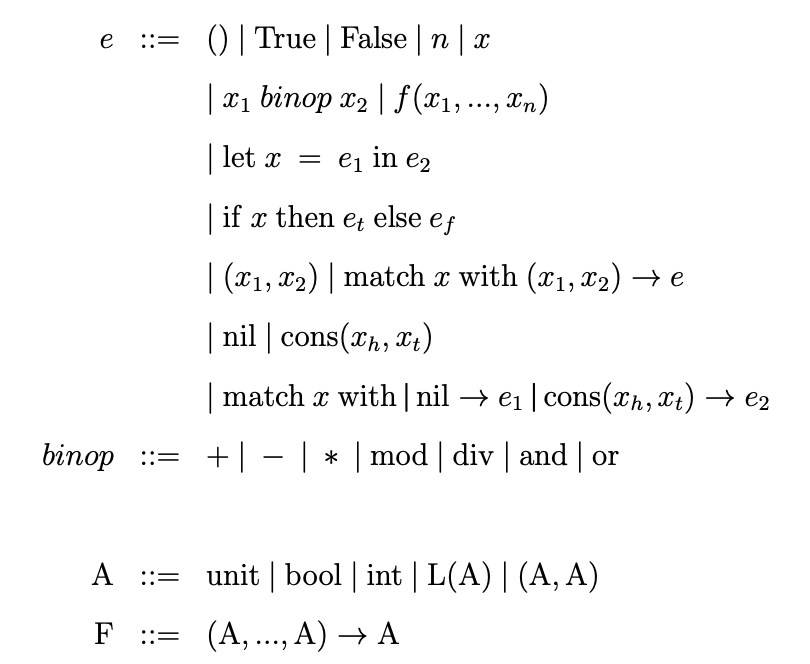
\includegraphics[scale=0.8]{image1.png}
    \caption{RAMLの文法}
    \label{image1}
  \end{center}
\end{figure}

\begin{comment}
\begin{eqnarray*}
  e &::=& ()\ {\rm |\ True\ |\ False}\ |\ n\ |\ x \\
  &&|\ x_1\ binop\ x_2\ |\ f(x_1,...,x_n) \\
  &&|\ {\rm let}\ x\ =\ e_1\ {\rm in}\ e_2 \\
  &&|\ {\rm if}\ x\ {\rm then}\ e_t\ {\rm else}\ e_f \\
  &&|\ (x_1,x_2)\ |\ {\rm match}\ x\ {\rm with}\ (x_1,x_2) \rightarrow e \\
  &&|\ {\rm nil\ |\ cons}(x_h,x_t) \\
  &&|\ {\rm match}\ x\ {\rm with \mbox{\boldmath |} nil} \rightarrow e_1 \mbox{\boldmath |}{\rm cons}(x_h,x_t) \rightarrow e_2 \\
  binop &::=& {\rm +\ |\ -\ |\ *\ |\ mod\ |\ div\ |\ and\ |\ or} \\
  \\
  {\rm A}&::=& {\rm unit\ |\ bool\ |\ int\ |\ L(A)\ |\ (A,A)} \\
  {\rm F}&::=& {\rm (A,...,A) \rightarrow A}
\end{eqnarray*}
\end{comment} 

図\ref{image1} にRAMLの文法を示す.$e$はRAMLプログラム上の式を表していて,
Unit値(),Boolean値True,False,整数値$n$,変数$x$,変数$x_1$と$x_2$の演算,
関数適用,let式を用いた局所関数を伴う式,ifによる条件分岐式,変数$x_1$と$x_2$のペア,
ペアに対するmatch式,空リストnil,リストの結合を表すcons$(x_h,x_t)$,リストに対するmatch式がある.
演算子$binop$には,整数値に対する演算である+,-,*,mod,div,
Boolean値に対する演算であるand,orがある.
AとFは,RAMLプログラム上でのsimple typeを表している.
Aはデータ型で,Unit型のunit,Boolean型のbool,整数型のint,simple typeの値のリスト,
simple typeの値のペアがある.
Fは関数型で,simple typeの値を受け取ってsimple typeの値を返す関数型を表している.
また,RAML上のwell-typedな式を,このsimple typeが割り当てられた式と定義している.

RAMLプログラムは,関数宣言のリストとmain式からなる.関数宣言は,関数の型宣言または関数の定義である.
それぞれの関数定義に対して型宣言を行うことができるが,プログラム内で型宣言が行われていない関数については,
プログラム実行時に型推論が行われる.main式はリソース消費量の分析の対象となる式で,プログラムの最後に記述する.


RAMLのリソース消費量の分析は,入力されたプログラムの,
big-step operational semanticsによる各評価ステップに対して一定のコストを割り当てるメトリックによって,
リソース消費量の計算を行う.
メトリックは以下の4つが存在する.
\begin{itemize}
  \item heapメトリックは,実行時に割り当てられたヒープセルの数を計算する.
  \item stepsメトリックは,実行時の評価ステップ数を計算する.
  \item tickメトリックは,ユーザーが定義したtick関数によるtick値を計算する.
  ユーザーは関数の定義中にRaml.tick(1.0)のような関数(tick関数)を定義することができる.
  tick関数が呼び出される度に,引数のfloat値に等しいリソース消費(tick値)が発生する.
  \item flipsメトリックは,フリップ関数によるフリップ数を計算する.
  本論文では扱わないため,詳細な説明は省略する.
\end{itemize}

ユーザーは分析を行う際にメトリックを指定することで,
自分の注目するリソースの消費量を分析の出力として得ることができる.

RAMLプログラムの例として,リストに対するクイックソートを行うプログラムであるquicksortの
コードをCode \ref{code2}に示す.
\\

\begin{lstlisting} [language=caml, caption=quicksort.raml, label=code2]
let rec append l1 l2 =
  match l1 with
    | [] -> l2
    | x::xs -> x::(append xs l2)

let rec partition f l =
  match l with
    | [] -> ([],[])
    | x::xs ->
      let (cs,bs) = partition f xs in
      Raml.tick(1.0);
      if f x then (cs,x::bs) else (x::cs,bs)

let rec quicksort gt = function
  | [] -> []
  | x::xs ->
      let ys, zs = partition (gt x) xs in
      append (quicksort gt ys) (x :: (quicksort gt zs))

let _ = quicksort (fun a b -> a <= b)  [9;8;7;6;5;4;3;2;1]
\end{lstlisting}

見てわかる通り,プログラムのコードの見た目はOCamlに近いが,20行目のlet \_ = ...の部分はOCamlには見られない表現である.
この式がmain式で,リソース消費量の分析の対象となる.
このプログラムは,append,partition,quicksortの3つの関数を定義し,
main式はquicksortの関数適用が記述されている.

1-4行目のappend関数は,2つのリストl1,l2を引数として受け取り,
それらを結合したリストを返す関数である.
6-12行目のpartition関数は,リストlと,lの要素の型の値を受け取ってbool型の値を返す関数fを引数として受け取り,
lの要素をfに関数適用したときの返り値によって2つのリストに分割する関数である.
11行目にtick関数であるRaml.tick(1.0)があり,結果としてlの要素の数だけ1.0のtick値が発生する.
14-18行目のquicksort関数は,リストlと,lの要素の型の値を2つ受け取ってbool型の値を返す関数gtを引数として受け取り,
lに対してクイックソートを実行する関数である.quicksortの定義中にappendとpartitionが用いられている.

RAMLのプログラムの実行において,主にevaluationとanalysisの2つの操作がある.

evaluationは,プログラムの評価を行い,main式の評価結果の返り値を出力する.
また,先述した4つのメトリックによるリソース消費量を計算し出力する.
evaluationは,./main eval [prog.raml]というコマンドによって実行される.
ここでprog.ramlは入力として用いるプログラムファイルである.

quicksort.ramlを入力としてevaluationを実行した結果を以下に示す.
\\

\begin{lstlisting} [basicstyle={\ttfamily\color{base}\scriptsize}]
$ ./main eval examples/quicksort.raml

Resource Aware ML, Version 1.5.0, June 2020

Typechecking expression ...
  Typecheck successful.
  Stack-based typecheck successful.

Evaluating expression ...

  Return value:
    [ 1; 2; 3; 4; 5; 6; 7; 8; 9 ]

  Evaluation steps: 1624.00
  Ticks:            36.00
  Heap space:       547.00
  Flips:            0.00

\end{lstlisting}

11-12行目に,main式の評価の返り値として,リスト[9;8;7;6;5;4;3;2;1]が正しくソートされた値が出力されている.
また,14-17行目に,上からsteps,ticks,heap,flipsと,
それぞれのメトリックによって計算されたリソース消費量の値が出力されている.

analysisは,指定されたメトリックに則ってプログラムのリソース消費量の範囲の解析を実行する.
解析の結果として,リソース消費量の範囲が,入力されたプログラムに依存する変数の多項式として出力される.
出力される範囲は,リソース消費量の上限,下限,または上限と下限が一致した定数リソース境界から選ぶことができる.
analysisは,./main analyze [mode] <metric> [<d1>] <d2> [-print (all | none | consume | level <lev> )] [-m] [prog.raml] [func\_name]というコマンドで実行される.
ここで,<>は指定必須のオプションで,[]は任意のオプションである.
modeは出力される境界のタイプをupper,lower,constantから選ぶ.指定しない場合はupperとなる.
metricは分析に用いるメトリックをheap,steps,ticks,flipsから選ぶ.
d1およびd2は,リソース消費量の境界の次数を指定する.分析は次数がd1,d1+1,...,d2の範囲で行われ,
出力される多項式もその範囲の次数となる.d1を指定しない場合,d1=d2として扱われる.
-printはプログラムにおいて実行された関数の型を出力する.-printにもいくつかのオプションがあり,
-print allは実行されたすべての関数の型を出力する.-print noneは型の出力をしない.
-print consumeは消費関数(?)の型を出力する.
-print level <lev>は式を構文木として見た際に深さが<lev>以下の関数の型を出力する.
-mは,指定するとモジュールモードとなり,main式の代わりにトップレベルで定義された関数の型をすべて出力する.
prog.ramlは入力として用いるプログラムファイルである.
func\_nameはモジュールモードでのみ指定することができるオプションで,指定した関数についてのみ型を出力する.

quicksort.ramlを入力として,mode=upper,metric=steps,d1=1,d2=4,
-print level 1とオプションを設定してanalysisを実行した結果を以下に示す.
\\

\begin{lstlisting}[basicstyle={\ttfamily\color{base}\scriptsize}]
$ ./main analyze steps 1 4 -print level 1 examples/quicksort.raml

Resource Aware ML, Version 1.5.0, June 2020

Typechecking expression ...
  Typecheck successful.
  Stack-based typecheck successful.

Analyzing expression ...

  Trying degree: 1, 2

  Function types:

== quicksort :

  [int -> int -> bool; int list] -> int list

  Non-zero annotations of the argument:
        35  <--  (*, [::(*); ::(*)])
        36  <--  (*, [::(*)])
         3  <--  (*, [])

  Non-zero annotations of result:

  Simplified bound:
     3 + 18.5*M + 17.5*M^2
   where
     M is the number of ::-nodes of the 2nd component of the argument

====

  Derived upper bound: 1624.00

  Mode:          upper
  Metric:        steps
  Degree:        2
  Run time:      0.14 seconds
  #Constraints:  638
\end{lstlisting}

11行目にTrying degree: 1,2とあるが,指定された次数の1,2,3,4の低い値から順に分析を行い,
次数が2のときに分析が成功したことを示している.指定された次数において分析が成功しない場合,その旨がエラーメッセージで表示される.
15-29行目には,main式で用いられた関数quicksortの分析の結果が示されている.
17行目にquicksortの型が示されている.[]中の型が引数の型で,複数ある場合は;で区切られている.
19-22行目に,引数のポテンシャル注釈が引数のデータ構造ごとに示されている.
このポテンシャル注釈に関する情報を多項式に変換したものが,26-29行目に示されている.
そして,33行目にmain式の上界の値が出力され,35-39行目に分析のオプションや計算時間,計算量が出力されている.


\section{RAMLでのMichelsonプログラムの実装}

\section{ガス消費量の解析の結果と考察}

\section{改善点}

\section{結論}\label{sec-conclusion}

\acknowledgments

\nocite{*}
\bibliographystyle{kuisunsrt}
\bibliography{main}

\end{document}